\addcontentsline{toc}{chapter}{Занятие 6. Формула полной вероятности. Формула Байеса}
\chapter*{Занятие 6. Формула полной вероятности. Формула Байеса}

\addcontentsline{toc}{section}{Контрольные вопросы и задания}
\section*{Контрольные вопросы и задания}

\subsubsection*{Приведите определение полной группы гипотез.}

Набор случайных событий $H_1, \dotsc, H_n$ называется полным набором гипотез, если выполнены следующие условия:
\begin{enumerate}
\item $P \left( H_i \right) > 0, \, i = \overline{1, n} $;
\item $H_i \cap H_j = \emptyset, \, i \neq j$ (они несовместны);
\item $ \bigcup \limits_{i=1}^n H_i = \Omega $.
\end{enumerate}

\subsubsection*{Запишите формулу для вычисления условной вероятности, формулу полной вероятности, формулу Байеса.}

Условная вероятность события $A$ при условии, что событие $B$ произошло --- это выражение
$$P \left( \left. A \right| B \right) =
\frac{P \left( A \cap B \right) }{P \left( B \right) }.$$

Формула полной вероятности: $P \left( A \right) = \sum \limits_{i=1}^n P \left( \left. A \right| H_i \right) P \left( H_i \right) $.

Формула Байеса:
$$P \left( \left. H_i \right| A \right) =
\frac{P \left( \left. A \right| H_i \right) P \left( H_i \right) }{ \sum \limits_{k=1}^n P \left( \left. A \right| H_k \right) P \left( H_k \right) }.$$

\subsubsection*{Когда применяется формула полной вероятности, формула Байеса?}

В формуле полной вероятности содержатся априорные вероятности. Формула Байеса переоценивает вероятности гипотез --- апостериорные вероятности.

\addcontentsline{toc}{section}{Аудиторные задачи}
\section*{Аудиторные задачи}

\subsubsection*{6.3}

\textit{Задание.} В первой урне находятся 1 белый и 4 красных шара, а во второй урне --- 2 белых и 7 красных шаров.
Из второй урны наугад вынули 1 шар и переложили её в первую урну.
После этого из первой урны наугад вынули 1 шар.
Найдите вероятность того, что этот шар окажется красным.

\textit{Решение.}
Введём событие $A =$ \{шар, вынутый из первой урны после перекладывания одного шара из другой урны, окажется красным\} и сделаем гипотезы о том,
какого цвета шар переложили: $H_1 =$ \{из второй урны переложили в первую белый шар\}, $H_2 =$ \{из второй урны переложили в первую красный шар\}.

Проверяем, что это полная группа гипотез:
$$P \left( H_1 \right) =
\frac{2}{9} >
0, \,
P \left( H_2 \right) =
\frac{7}{9} >
0.$$
События не могут произойти одновременно.
$P \left( H_1 \right) + P \left( H_2 \right) =
1$.
Поэтому имеем полную группу гипотез.

Найдём условные вероятности:
$$P \left( \left. A \right| H_1 \right) =
\frac{4}{6}, \,
P \left( \left. A \right| H_2 \right) =
\frac{5}{6}.$$

Значит по формуле полной вероятности:
\begin{equation*}
\begin{split}
P \left( A \right) =
P \left( H_1 \right) P \left( \left. A \right| H_1 \right) + P \left( H_2 \right) P \left( \left. A \right| H_2 \right) =
\frac{2}{9} \cdot \frac{4}{6} + \frac{7}{9} \cdot \frac{5}{6} = \\
= \frac{2}{9} \cdot \frac{2}{3} + \frac{7}{9} \cdot \frac{5}{6} =
\frac{4}{27} + \frac{35}{54} =
\frac{8+35}{54} =
\frac{43}{54}.
\end{split}
\end{equation*}

\subsubsection*{6.4}

\textit{Задание.} Из урны, которая содержит 3 чёрных и 2 белых шара, наугад вынуты два шара и переложены в другую урну, которая содержит 4 чёрных и 4 белых шара.
Найдите вероятность того, что:
\begin{enumerate}[label=\alph*)]
\item шар, вынутый после этого наугад из второй урны, окажется белым;
\item из первой урны переложили в другую два чёрных шара, при условии, что шар, вынутый после этого из второй урны, оказался белым.
\end{enumerate}

\textit{Решение.} В первой урне содержится 3 чёрных и 2 белых шара, во второй --- 4 чёрных и 4 белых.
\begin{enumerate}[label=\alph*)]
\item Введём событие $A =$ \{вынутый из второй урны после переложения шар окажется белым\}.

Есть 3 разные гипотезы: $H_1 =$ \{переложили 2 белых шара\}, $H_2 = \\ =$ \{переложили 2 чёрных шара\}, $H_3 =$ \{переложили 1 белый и 1 чёрный шар\}.

Находим вероятности этих гипотез:
\begin{equation*}
\begin{split}
P \left( H_1 \right) =
\frac{C_2^2}{C_5^2} =
\frac{2! \cdot 3!}{5!} = 
\frac{2 \cdot 2 \cdot 3}{2 \cdot 3 \cdot 4} =
\frac{1}{2 \cdot 5} =
\frac{1}{10} >
0; \\
P \left( H_2 \right) =
\frac{C_3^2}{C_5^2} =
\frac{3!}{2!} \cdot \frac{2! \cdot 3!}{5!} =
\frac{3}{10} >
0; \\
P \left( H_3 \right) =
\frac{C_3^1 \cdot C_2^1}{C_5^2} =
\frac{3 \cdot 2 \cdot 2 \cdot 2 \cdot 3}{2 \cdot 3 \cdot 4 \cdot 5} =
\frac{3}{5} >
0.
\end{split}
\end{equation*}

В сумме вероятности гипотез дают единицу.
Гипотезы не могут одновременно происходит, поэтому они являются полным набором гипотез.

Найдём условные вероятности:
$$P \left( \left. A \right| H_1 \right) =
\frac{6}{10}, \,
P \left( \left. A \right| H_2 \right) =
\frac{4}{10}, \,
P \left( \left. A \right| H_3 \right) =
\frac{1}{2}.$$

По формуле полной вероятности:
\begin{equation*}
\begin{split}
P \left( A \right) =
\frac{1}{10} \cdot \frac{6}{10} + \frac{2}{10} \cdot \frac{4}{10} + \frac{3}{5} \cdot \frac{1}{2} =
\frac{1}{10} \cdot \frac{3}{5} + \frac{3}{10} \cdot \frac{2}{5} + \frac{3}{5} \cdot \frac{1}{2} = \\
= \frac{3}{50} + \frac{6}{50} + \frac{3}{10} =
\frac{3+6+15}{50} =
\frac{24}{50} =
\frac{12}{25};
\end{split}
\end{equation*}

\item $A$ стало условием.
Знаем, что это событие произошло.
По формуле Байеса:
\begin{equation*}
\begin{split}
P \left( \left. H_2 \right| A \right) =
\frac{P \left( H_2 \right) P \left( \left. A \right| H_2 \right) }{P \left( H_1 \right) P \left( \left. A \right| H_1 \right) +
P \left( H_2 \right) P \left( \left. A \right| H_2 \right) + P \left( H_3 \right) P \left( \left. A \right| H_3 \right) } = \\
= \frac{P \left( H_2 \right) P \left( \left. A \right| H_2 \right) }{P \left( A \right) } =
\frac{3}{10} \cdot \frac{4}{10} \cdot \frac{25}{12} =
\frac{1}{4}.
\end{split}
\end{equation*}
\end{enumerate}

\subsubsection*{6.5}

\textit{Задание.} Некоторое изделие выпускается двумя заводами, причём объём продукции первого завода в 3 раза больше объёма продукции второго завода.
Доля бракованных изделий составляет $0.1$ на первом заводе, и $0.05$ --- на втором.
Изделия, выпущенные обоими заводами за одинаковый промежуток времени, смешали и пустили в продажу.
Вы приобрели такое изделие.
Найдите вероятность того, что изделие было изготовлено на первом заводе, если оно окажется:
\begin{enumerate}[label=\alph*)]
\item качественным;
\item бракованным.
\end{enumerate}

\textit{Решение.}
\begin{enumerate}[label=\alph*)]
\item Это задача на формулу Байеса.
Нам известно, что изделие оказалось качественным: $A =$ \{изделие оказалось качественным\}.
Гипотезы: $H_1 =$ \{изготовили это изделие на первом заводе\}, $H_2 =$ \{это изделие изготовили на втором заводе\}.
Нужно найти $P \left( \left. H_1 \right| A \right) $.
Вероятности гипотез:
$$P \left( H_1 \right) =
\frac{3}{4}, \,
P \left( H_2 \right) =
\frac{1}{4}.$$
Условные вероятности: $P \left( \left. A \right| H_1 \right) = 0.9, \, P \left( \left. A \right| H_2 \right) = 0.095$.
По формуле полной вероятности:
\begin{equation*}
\begin{split}
P \left( A \right) =
P \left( H_1 \right) P \left( \left. A \right| H_1 \right) + P \left( H_2 \right) P \left( \left. A \right| H_2 \right) =
\frac{3}{4} \cdot 0.9 + \frac{1}{4} \cdot 0.95 = \\
= \frac{3}{4} \cdot \frac{9}{10} + \frac{1}{4} \cdot \frac{95}{100} =
\frac{27}{40} + \frac{95}{100} =
\frac{365}{400} =
\frac{73}{80}.
\end{split}
\end{equation*}
Применяем формулу Байеса:
$$P \left( \left. H_1 \right| A \right) =
\frac{P \left( \left. A \right| H_1 \right) P \left( H_1 \right) }{P \left( A \right) } =
\frac{9}{10} \cdot \frac{3}{4} \cdot \frac{80}{73} =
\frac{27 \cdot 2}{73} =
\frac{54}{73};$$
\item введём событие $B =$ \{изделие оказалось бракованным\}.
Условные вероятности: $P \left( \left. B \right| H_1 \right) = 0.1, \, P \left( \left. B \right| H_2 \right) = 0.05$.
События $A$ и $B$ --- противоположные:
$$P \left( B \right) =
1 - P \left( A \right) =
1 - \frac{73}{80} =
\frac{7}{80}.$$
По формуле Байеса:
$$P \left( \left. H_1 \right| B \right) = \frac{ \left( \left. B \right| H_1 \right) P \left( H_1 \right) }{P \left( B \right) } =
\frac{1}{10} \cdot \frac{3}{4} \cdot \frac{80}{7} =
\frac{3 \cdot 2}{7} =
\frac{6}{7}.$$
\end{enumerate}

\subsubsection*{6.6}

\textit{Задание.} Три приятеля --- Андрей, Борис и Володя --- пришли в тир.
Андрей попадает в мишень с вероятностью $3/5$, Борис --- с вероятностью $1/2$, а Володя --- с вероятностью $2/5$.
Одновременно они выстрелили по мишени и две пули попали.
Что вероятнее: попал Володя в мишень или нет?

\textit{Решение.} Введём событие $A =$ \{2 выстрела из трёх оказались точными\}.
Введём гипотезы: $H_1 =$ \{Володя попал\}, $H_2 =$ \{Володя не попал\}.
Их вероятности равны
$$P \left( H_1 \right) =
\frac{2}{5}, \,
P \left( H_2 \right) =
\frac{3}{5}.$$
Условные вероятности: $P \left( \left. A \right| H_1 \right) = P$ (\{или Андрей попал, Борис --- нет, или Андрей не попал, а Бори попал\}).
События несовместные.
$$P \left( \left. A \right| H_1 \right) =
\frac{3}{5} \cdot \frac{1}{2} + \frac{2}{5} \cdot \frac{1}{2} =
\frac{3}{10} + \frac{2}{10} =
\frac{1}{2};$$
$P \left( \left. A \right| H_2 \right) = P$ (\{Андрей и Борис попали\}) $= \frac{3}{5} \cdot \frac{1}{2} = \frac{3}{10}.$

По формуле Байеса:
$$P \left( \left. H_1 \right| A \right) =
\frac{1}{2} \cdot \frac{2}{5} \cdot \frac{1}{P \left( A \right) } =
\frac{1}{5P \left( A \right) }, \,
P \left( \left. H_2 \right| A \right) =
\frac{3}{5} \cdot \frac{3}{10} \cdot \frac{1}{P \left( A \right) } =
\frac{9}{50 P \left( A \right) }.$$
Имеем, что $P \left( \left. H_1 \right| A \right) > P \left( \left. H_2 \right| A \right) \Rightarrow $ более вероятно,
что Володя попал при этих двух точных выстрелах.

\subsubsection*{6.7}

\textit{Задание.}
Группа студентов, которые сдают экзамен,
состоит из 5 отличников,
10 хороших студентов и 15 слабых студентов;
отличник всегда получает оценку <<отлично>>,
хороший студент ---
оценки <<отлично>> и <<хорошо>> с одинаковыми вероятностями,
слабый студент --- <<хорошо>> и <<удовлетворительно>> или <<неудовлетворительно>> с одинаковыми вероятностями.
Найдите вероятность того, что наугад выбранный студент получит оценку:
\begin{enumerate}[label=\alph*)]
\item <<отлично>>;
\item <<хорошо>>.
\end{enumerate}

\textit{Решение.}
\begin{enumerate}[label=\alph*)]
\item Введём событие $A =$ \{наугад выбранный студент получит <<отлично>>\}.
Сделаем гипотезы: $H_1 =$ \{выбранный студент --- отличник\},
$H_2 =$ \{выбранный студент --- хороший\}, $H_3 =$ \{выбранный студент --- слабый\}.
Их вероятности равны:
$$P \left( H_1 \right) =
\frac{5}{30} =
\frac{1}{6}, \,
P \left( H_2 \right) =
\frac{10}{30} =
\frac{1}{3}, \,
P \left( H_3 \right) =
\frac{15}{30} =
\frac{1}{2}.$$
Условные вероятности:
$$P \left( \left. A \right| H_1 \right) =
1, \,
P \left( \left. A \right| H_2 \right) =
\frac{1}{2}, \,
P \left( \left. A \right| H_3 \right) =
0.$$
Таким образом,
$$P \left( A \right) =
\frac{1}{6} + \frac{1}{3} \cdot \frac{1}{2} =
\frac{1}{3};$$
\item введём событие $B =$ \{студент получает <<хорошо>>\}.
Условные вероятности:
$$P \left( \left. B \right| H_1 \right) =
0, \,
P \left( \left. B \right| H_2 \right) =
\frac{1}{2}, \,
P \left( \left. B \right| H_3 \right) =
\frac{1}{3}.$$
Таким образом,
$$P \left( B \right) =
0 \cdot \frac{1}{6} + \frac{1}{2} \cdot \frac{1}{3} + \frac{1}{3} \cdot \frac{1}{2} =
\frac{1}{3}.$$
\end{enumerate}

\subsubsection*{6.8}

\textit{Задание.}
Допустим,
что частоты генотипов $AA, Aa$ и $aa$ в некоторой популяции равны $p^2, 2pq$ и $q^2$ соответственно ($p+q = 1$,
генотипы $Aa$ и $aA$ считаются одинаковыми).
Известно, что кто-то имеет генотип $Aa$.
Докажите, что вероятность того, что генотип его брата тоже $Aa$, равна $ \left( 1+pq \right) /2$.

\textit{Решение.} $AA$ --- доминантный генотип, $aa$ --- рецессивный, $Aa$ --- гибридный.

Братья имеют одних и тех же родителей.
Допустим, мама имеет генотип $AA$, а папа --- $Aa$.
Возможные случаи для ребёнка: $AA, Aa$.

Каждая буква выбирается с вероятностью $1/2$.
Если зафиксировать генотипы родителей, то генотипы братьев будут условно независимыми.
Но они зависимы через родителей.

Частоты генотипов: $AA = p^2, Aa = 2qp, aa = q^2$, где $p + q = 1$.

Пусть событие  $B =$ \{генотип одного из братьев --- $Aa$\}.
Введём гипотезы:
\begin{center}
    \begin{tabular}{| l | l | l | l | l |}
    \hline
    Гипотеза & Генотип 1 & Генотип 2 & $P \left( H_i \right)$ & $P \left( \left. B \right| H_i \right)$ \\ \hline
    $H_1$ & $AA$ & $AA$ & $p^4$ & 0 \\ \hline
    $H_2$ & $AA$ & $Aa$ & $2p^3 q$ & $ \frac{1}{4} $ \\ \hline
    $H_3$ & $AA$ & $aa$ & $p^2 q^2$ & 1 \\ \hline
    $H_4$ & $Aa$ & $AA$ & $2p^3 q$ & $ \frac{1}{4} $ \\ \hline
    $H_5$ & $Aa$ & $Aa$ & $4p^2 q^2$ & $ \frac{1}{4} $ \\ \hline
    $H_6$ & $Aa$ & $aa$ & $2pq^3$ & $ \frac{1}{4} $ \\ \hline
    $H_7$ & $aa$ & $AA$ & $p^2 q^2$ & 1 \\ \hline
    $H_8$ & $aa$ & $Aa$ & $2pq^3$ & $ \frac{1}{4} $ \\ \hline
    $H_9$ & $aa$ & $aa$ & $q^4$ & 0 \\ \hline
    \end{tabular}
\end{center}

Перемножаем 2 последних столбца и складываем.
Получим вероятность того, что у обоих братьев генотипы $Aa$:
\begin{equation*}
\begin{split}
2p^3 q \cdot \frac{1}{4} +
p^2 q^2 \cdot 1 +
2p^3 q \cdot \frac{1}{4} + 4p^2 q^2 \cdot \frac{1}{4} + 2p q^3 \cdot \frac{1}{4} + p^2 q^2 \cdot 1 + 2pq^3 \cdot \frac{1}{4} = \\
= p^3 q + 3p^2 q^2 + pq^3 =
pq \left( p^2 + 3pq + q^2 \right) =
pq \left[ \left( p^2 + 2pq + q^2 \right) + pq \right] = \\
= pq \left( 1 + pq \right).
\end{split}
\end{equation*}

Тогда вероятность равна:
$$ \frac{pq \left( 1+pq \right) }{2pq} =
\frac{1+pq}{2}.$$

\subsubsection*{6.9}

\textit{Задание.} Частица совершает случайное симметрическое блуждание на числовой оси, делая шаг вправо или влево с вероятностью $1/2$.
Найдите вероятность того, что частица, которая стартовала из точки $x$, рано или поздно попадёт в точку $0$.

\textit{Решение.} Из каждой точки частица с одинаковой вероятностью перемещается вправо и влево (рис. \ref{fig:69}).

\begin{figure}[h!]
  \centering
  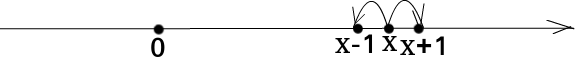
\includegraphics[width=.4\textwidth]{./pictures/6_9.png}
  \caption{Возможные движения частицы}
  \label{fig:69}
\end{figure}

Частица перемещается на шаг вправо или влево.
Получаем аналогичную задачу для $x + 1$ или $x - 1$.

Пусть $f \left( x \right) $ --- вероятность того, что частица из $x$ попала в 0.
Введём гипотезы: $H_1 =$ \{частица сделает шаг вправо из точки $x$\}, $H_2 =$ \{частица сделает шаг право из точки $x$\}.
Введём событие $A =$ \{частица из $x$ перейдёт в 0\}.
Вероятности гипотез равны
$$P \left( H_1 \right) =
P \left( H_2 \right) =
\frac{1}{2}.$$
По формуле полной вероятности:
$$P \left( A \right) =
\frac{1}{2} \cdot P \left( \left. A \right| H_1 \right) + \frac{1}{2} P \left( \left. A \right| H_2 \right).$$
Имеем уравнение:
$$f \left( x \right) =
\frac{1}{2} \cdot f \left( x+1 \right) + \frac{1}{2} \cdot f \left( x-1 \right).$$
Уравнение описывает прямую $f \left( x \right) = ax + b$.
Поскольку $f \left( 0 \right) = 1$, значит $b = 1$.
Значит $f \left( x \right) = ax + 1$.
Вероятность $f \left( x \right) \in \left[ 0, 1 \right] $.
Только прямая $y = 1$ (\ref{fig:691}) удовлетворяет условию $f \left( x \right) \leq 1 \Rightarrow a = 0$.

\begin{figure}[h!]
  \centering
  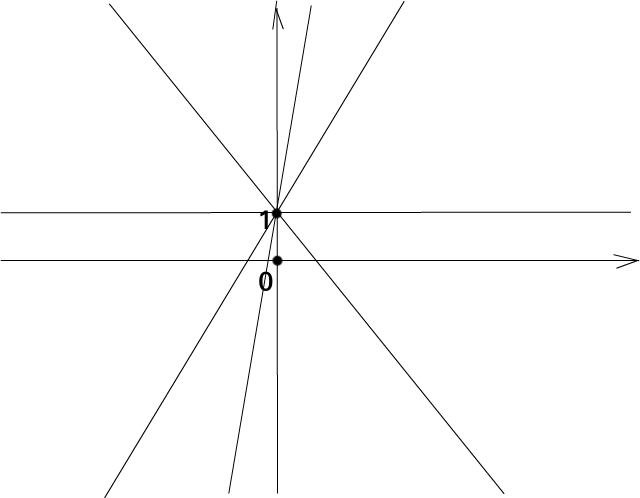
\includegraphics[width=.4\textwidth]{./pictures/6_9_1.png}
  \caption{Возможные движения частицы}
  \label{fig:691}
\end{figure}

Таким образом $f \left( x \right) = 1$.

\subsubsection*{6.10}

\textit{Задание.}
Рассмотрим последовательность независимых экспериментов,
в каждом из которых некоторое событие ---
<<успех>> происходит с вероятностью $p$, а противоположное событие --- <<неудача>> --- происходит с вероятностью $q = 1 - p$.
Найдите вероятность того, что два последовательных <<успеха>> произойдут раньше трёх последовательных <<неудач>>.

\textit{Решение.} Следим за событием, которое заканчивается <<успехом>> или <<неудачей>>.
Количество экспериментов не ограничено.
Введём гипотезы: $H_1 =$ \{первым был <<успех>>\}, $H_2 =$ \{первой была <<неудача>>\}.
Условные вероятности: $x = P \left( \left. A \right| H_1 \right), \, y = p \left( \left. A \right| H_2 \right) $.
Основное событие $A =$ \{2 последовательных <<успеха>> произойдут раньше чем 3 последовательные <<неудачи>>\}.
Вероятности гипотез: $P \left( H_1 \right) = p$, а $P \left( H_2 \right) = q = 1 - p$.
Вероятность того, что событие $A$ произойдёт при том,
что первый эксперимент завершился <<успехом>>,
равна
$P \left( \left. A \right| <<y>> \right) =
P \left( \left. A \right| <<yy>> \right) P$(<<успех>> во втором эксперименте)$+ P$ (<<неудача>> во втором эксперименте)$P \left( \left. A \right| <<yn>> \right) = \\ = x$.
Вероятность того, что произойдёт событие $A$ при том, что в первом эксперименте будет <<неудача>>, равна $P \left( \left. A \right| <<n>> \right) = y$.
Условная вероятность события $A$ при условии, что первый эксперимент завершился <<успехом>>, равна $x = p \cdot 1 + \left( 1-p \right) y$, где $y = p \left( 1-p \right) y + p^2 + \left( 1-p \right) px$.
Есть система уравнений:
$$
\begin{cases}
x = p + \left( 1-p \right) y,\\
y = p \left( 1-p \right) y + p^2 + \left( 1-p \right) px.\\
\end{cases}
$$
Подставим $x$, получим уравнение относительно $y: \, P \left( A \right) = px + qy$.

\subsubsection*{6.11}

\textit{Задание.} Подводная лодка атакует корабль, выпуская по нему последовательно и независимо друг за другом $n$ торпед.
Каждая торпеда попадает в корабль с вероятностью $p$ и, попав, ---
з одинаковыми вероятностями поражает один из $m$ отсеков, на которые разделена подводная часть корабля.
Корабль идёт на дно, если поражено не меньше двух отсеков.
Найдите вероятность того, что корабль потопят.

\textit{Решение.} Введём событие $A =$ \{корабль потопят\}.

Введём гипотезы $H_i =$ \{в корабль попало $i$ торпед\}, $i = 0, 1, 2, \dotsc, n$.
Условные вероятности события $A$ при том, что в корабль попадёт 0 или 1 торпеда,
равны $P \left( \left. A \right| H_0 \right) = 0, \, P \left( \left. A \right| H_1 \right) = 0$.
Рассмотрим вероятности того, что в 1 отсек попало $i$ торпед: $1/m^2$ ---
вероятность затопления одного и того же отсека при попадании двух торпед,
$1/m^3$ ---
вероятность затопления одного и того же отсека при попадании трёх торпед,
$ \dotsc, 1/m^3$ --- вероятность затопления одного и того же отсека при попадании $n$ торпед.

Предположим, что в корабль попало $t$ торпед.
При этом: первая торпеда попала в один и тот же отсек, что и другие (а других пока нет) с вероятностью 1, 2-ая после 1-ой ракеты --- с вероятностью $1/m$, 3-ая после 2-ой --- с вероятностью $1/m^2, \dotsc, t$-ая с вероятностью $1/m^{t-1}$.

Следовательно:
$$P \left( \left. A \right| H_t \right) =
1 - \frac{1}{m^{t-1}}, \, t \leq 1;$$

По формуле полной вероятности:
\begin{equation*}
\begin{split}
P \left( A \right) =
C_n^2 p^2 q^{n-2} \left( 1 - \frac{1}{m} \right) +
C_n^3 p^3 q^{n-3} \left( 1 - \frac{1}{m^2} \right) + \dotsc + \\
+ C_n^n p^n \left( 1 - \frac{1}{m^n} \right) =
\sum \limits_{i=2}^n C_n^i p^i q^{n-i} \left( 1 - \frac{1}{m^{i-1}} \right).
\end{split}
\end{equation*}

\addcontentsline{toc}{section}{Дополнительные задачи}
\section*{Дополнительные задачи}

\subsubsection*{6.12}

\textit{Задание.} В волейболе команда может получить очко только на собственной подаче.
Поэтому каждая подача заканчивается или получением одного очка командой, которая подавала мяч, или переходом подачи другой команде.
Выигрывает та команда, которая первой получит $N$ очков.
Допустим, что команды имеют одинаковую вероятность $p > 0$ получить очко на собственной подаче.
Покажите, что в этом случае команда, которая подаёт первой, имеет большие шансы на выигрыш.
(Указание: введите в рассмотрение вероятность $p'$ того, что команда получит следующее очко, при условии, что она подаёт).

\textit{Решение.} Вероятность того, что команда получит очко при своей подаче равна $p$.
Если эта команда не получает очко при подаче, то подача переходит другой команде --- вероятность равна $1 - p$.

Есть такие состояния: $A_1$ --- команда $А$ забила, $A_0$ --- перешёл мяч команде $B$, $B_1$ --- команда $B$ забила, $B_0$ --- перешёл мяч команде $А$.

Начальное состояние --- у команды $А$ мяч --- состояние $A$.
При этом $P \left( B_1 \right) = P \left( B_0 \right) = 0$.
Нужно составить матрицу переходов.
Строки --- текущее состояние, колонки --- то, в которое можно перейти.

\begin{center}
    \begin{tabular}{| l | l | l | l | l | l | l |}
    \hline
    & $A$ & $A_1$ & $A_0$ & $B$ & $B_1$ & $B_0$ \\ \hline
    $A$ & 0 & $p$ & $1 - p$ & 0 & 0 & 0 \\ \hline
    $A_1$ & 1 & 0 & 0 & 0 & 0 & 0 \\ \hline
    $A_0$ & 0 & 0 & 0 & 1 & 0 & 0 \\ \hline
    $B$ & 0 & 0 & 0 & 0 & $p$ & $1 - p$ \\ \hline
    $B_1$ & 0 & 0 & 0 & 1 & 0 & 0 \\ \hline
    $B_0$ & 1 & 0 & 0 & 0 & 0 & 0 \\ \hline
    \end{tabular}
\end{center}

Команды работают абсолютно одинаково.
Если игра начнётся в состоянии $A$,
то вероятность пройти $N$ раз через состояние $А_1$ такая же как начать игру в состоянии $B$ и пройти $N$ раз через состояние $B_1$.
Начали в состоянии $A$.
Пусть есть вероятность $p_A^N$ того, что команда $A$ начала и забила первая $N$ голов.
Тогда с вероятностью $p \cdot p_A^{N-1}$ она забьёт $N$ голов при условии, что в первый раз она забила.
Вероятность того, что команда $B$ первой забьёт $N$ голов обозначим $p_B^N = p_A^N \left( 1-p \right) + p^k \left( 1-p \right) x$,
где $k$ --- количество голов, которые успела забить команда $A$, а это не меньше чем $p_A^N$, $x$ --- вероятность того, что команда $B$ забьёт первая $N$ голов при условии, что команда $A$ уже забила $k$ голов.

\addcontentsline{toc}{section}{Домашнее задание}
\section*{Домашнее задание}

\subsubsection*{6.13}

\textit{Задание.} В первой урне содержатся 1 белый и 9 чёрных шаров; во второй урне --- 1 чёрный и 5 белых шаров.
Из каждой урны наугад вынуто по одному шару, а остальные пересыпали в третью урну.
Найдите вероятность того, что шар, вынутый наугад из третьей урны, окажется белым.

\textit{Решение.}
Введём полную группу гипотез:
$H_1 =$ \{из обеих урн вынули по одному белому шару\};
$H_2 =$ \{из первой урны достали 1 белый шар и из второй --- 1 чёрный шар\};
$H_3 =$ \{из обеих урн вынули по одному чёрному шару\};
$H_4 =$ \{из первой урны достали 1 чёрный шар и из второй урны --- 1 белый шар\}.
Определим вероятности этих гипотез:
\begin{equation*}
\begin{split}
P \left\{ H_1 \right\} =
\frac{1}{10} \cdot \frac{5}{6} =
\frac{1}{12}, \,
P \left\{ H_2 \right\} =
\frac{1}{10} \cdot \frac{1}{6} =
\frac{1}{60}, \,
P \left\{ H_3 \right\} =
\frac{9}{10} \cdot \frac{1}{6} =
\frac{3}{10 \cdot 2} =
\frac{3}{20}, \\
P \left\{ H_4 \right\} =
\frac{9}{10} \cdot \frac{5}{6} =
\frac{3}{4}.
\end{split}
\end{equation*}
Введём событие $A =$ \{из третьей урны вытянули белый шар\}.
В то же время
$$P \left\{ \left. A \right| H_1 \right\} =
\frac{4}{14} =
\frac{2}{7}, \,
P \left\{ \left. A \right| H_2 \right\} =
\frac{5}{14} =
P \left\{ \left. A \right| H_4 \right\}, \,
P \left\{ \left. A \right| H_3 \right\} =
\frac{6}{14} =
\frac{3}{7}.$$
Согласно с формулой полной вероятности $P \left\{ A \right\} = \sum \limits_{i=1}^\infty P \left\{ H_i \right\} \cdot P \left\{ \left. A \right| H_i \right\} $ имеем
\begin{equation*}
\begin{split}
P \left\{ A \right\} =
\frac{1}{12} \cdot \frac{2}{7} + \frac{1}{60} \cdot \frac{5}{14} + \frac{3}{20} \cdot \frac{3}{7} + \frac{3}{4} \cdot \frac{5}{14} =
\frac{38}{105}.
\end{split}
\end{equation*}

\subsubsection*{6.14}

\textit{Задание.} Два стрелка стреляют по мишени.
Один из них попадает в 5 случаях, а другой --- в 8 случаях из 10.
Перед выстрелом они подбрасывают правильную монету для определения очередности.
Сторонний наблюдатель знает условия стрельбы, но не видит, кто в данный момент стреляет.
Он видит, что стрелок попал по мишени.
Найдите вероятность того, что стрелял первый стрелок.

\textit{Решение.} Первый стрелок попадает по мишени с вероятностью
$$P \left( \left. A \right| H_1 \right) =
\frac{5}{10} =
\frac{1}{2},$$
второй стрелок --- с вероятностью
$$P \left( \left. A \right| H_2 \right) =
\frac{8}{10} =
\frac{4}{5}.$$
Априорные вероятности этих гипотез одинаковы:
$$P \left( H_1 \right) =
P \left( H_2 \right) =
\frac{1}{2}.$$
Рассмотрим событие $A =$ \{стрелок попал в цель\}.
Поэтому вероятность стрелять первому стрелку по формуле Байеса равна
\begin{equation*}
\begin{split}
P \left( \left. H_1 \right| A \right) =
\frac{P \left( \left. A \right| H_1 \right) P \left( H_1 \right) }{P \left( \left. A \right| H_1 \right) P \left( H_1 \right) +
P \left( \left. A \right| H_2 \right) P \left( H_2 \right) } =
\frac{ \frac{1}{2} \cdot \frac{1}{2} }{ \frac{1}{2} \cdot \frac{1}{2} + \frac{4}{5} \cdot \frac{1}{2} } =
\frac{ \frac{1}{4} }{ \frac{1}{4} + \frac{2}{5} } = \\
= \frac{ \frac{1}{4} }{ \frac{5+8}{20} } =
\frac{20}{4 \cdot 13} =
\frac{5}{13}.
\end{split}
\end{equation*}

\subsubsection*{6.15}

\textit{Задание.} Среди $N$ экзаменационных билетов есть $n$ <<счастливых>>.
Студенты подходят за билетами по одному.
У кого больше шансов вынуть счастливый билет: у того, кто подошёл первым, или у того, что подошёл вторым?
Найдите вероятность того, что студент, который подошёл первым, вынул счастливый билет, если известно, что студент, который подошёл вторым, вынул счастливый билет.

\textit{Решение.} Если студент сдаёт экзамен первым, то вероятность вынуть счастливый билет равна $n/N$.
Рассмотрим ситуацию, когда он сдаёт вторым.
Введём гипотезы: $H_1$ --- первый забрал <<счастливый>> билет, $H_2$ --- первый не забрал <<счастливый>> билет.
Событие $A =$ \{студент сдал экзамен\}.
\begin{equation*}
\begin{split}
P \left( \left. A \right| H_1 \right) =
\frac{n-1}{N-1}, \,
P \left( \left. A \right| H_2 \right) =
\frac{n}{N-1}, \,
P \left( H_1 \right) =
\frac{n}{N}, \,
P \left( H_2 \right) =
1 - \frac{n}{N} = \\
= \frac{N-n}{N}.
\end{split}
\end{equation*}
Используем формулу полной вероятности:
\begin{equation*}
\begin{split}
P \left( A \right) =
\frac{n-1}{N-1} \cdot \frac{n}{N} + \frac{n}{N-1} \cdot \frac{N-n}{N} =
\frac{n}{N \left( N-1 \right) } \cdot \left( n-1+N-n \right) = \\
= \frac{n \left( N-1 \right) }{N \left( N-1 \right) } =
\frac{n}{N}.
\end{split}
\end{equation*}
Вывод: без разницы, когда сдавать.

Вероятность того, что студент, который пошёл первым, вынул счастливый билет, если известно, что студент, который пошёл вторым, вынул счастливый билет:
\begin{equation*}
\begin{split}
P \left( \left. H_1 \right| A \right) =
\frac{P \left( \left. A \right| H_1 \right) P \left( H_1 \right) }{P \left( \left. A \right| H_1 \right) P \left( H_1 \right) +
P \left( \left. A \right| H_2 \right) P \left( H_2 \right) } = \\
= \frac{ \frac{n-1}{N-1} \cdot \frac{n}{N} }{ \frac{n-1}{N-1} \cdot \frac{n}{N} + \frac{n}{N-1} \cdot \frac{N-n}{N} } =
\frac{ \frac{n-1}{N-1} \cdot \frac{n}{N} }{ \frac{n}{N \left( N-1 \right) } \cdot \left( n-1+N-n \right) } =
\frac{n-1}{N-1}.
\end{split}
\end{equation*}

\subsubsection*{6.16}

\textit{Задание.} На вход радиолокационного устройства с вероятностью $0.4$ попадает сигнал с шумом и с вероятностью $0.6$ --- только шум.
Если попадает сигнал с шумом, то устройство регистрирует наличие сигнала с вероятностью $0.7$, а если попадает только шум,
то устройство регистрирует наличие сигнала с вероятностью $0.5$.
Известно, что устройство зарегистрировало сигнал.
Найдите вероятность того, что сигнал действительно попал на вход радиолокационного устройства.

\textit{Решение.}
Введём событие $A =$ \{устройство зарегистрировало наличие сигнала\} и сделаем гипотезы о том,
какой же сигнал попал на радиолокационное устройство: $H_1 =$ \{попал сигнал с шумом\}, $H_2 =$ \{попал только шум\}.
Нам нужно найти условную вероятность $P \left( \left. H_1 \right| A \right) $.
По формуле Байеса:
\begin{equation*}
\begin{split}
P \left( \left. H_1 \right| A \right) =
\frac{P \left( \left. A \right| H_1 \right) P \left( H_1 \right) }{P \left( \left. A \right| H_1 \right) P \left( H_1 \right) +
P \left( \left. A \right| H_2 \right) P \left( H_2 \right) } =
\frac{0.7 \cdot 0.4}{0.7 \cdot 0.4 + 0.5 \cdot 0.6} = \\
= \frac{7 \cdot 4}{7 \cdot 4 + 5 \cdot 6} =
\frac{7 \cdot 2}{7 \cdot 2 + 5 \cdot 3} =
\frac{14}{14 + 15} =
\frac{14}{29}.
\end{split}
\end{equation*}

\subsubsection*{6.17}

\textit{Задание.} В Лондоне в половину дней года идёт дождь.
Прогноз погоды сбывается в $2/3$ случаев,
то есть условная вероятность того,
что будет идти дождь, при условии, что его прогнозировали, и условная вероятность того, что дождя не будет, при условии, что его не прогнозировали, равны $2/3$.
Если прогнозируют дождь, мистер Пиквик всегда берёт зонт.
Если же дождь не прогнозируют, то мистер Пиквик берёт зонт с вероятностью $1/3$.
Найдите вероятность того, что:
\begin{enumerate}[label=\alph*)]
\item мистер Пиквик не имеет зонта, при условии, что идёт дождь;
\item дождя нет, при условии, что мистер Пиквик имеет зонт.
\end{enumerate}

\textit{Решение.}
Выберем событие $A =$ \{мистер Пиквик берёт зонт\} и сделаем гипотезы о том,
будет или нет дождь, прогнозировали его или нет: $H_1 = \\ =$ \{дождь прогнозировали\}, $H_2 =$ \{дождь не прогнозировали\}, $X_1 =$ \{идёт дождь\}, $X_2 =$ \{дождь не идёт\}.
Есть такие условия:
\begin{equation*}
\begin{split}
P \left( X_1 \right) =
P \left( X_2 \right) =
\frac{1}{2}, \,
P \left( \left. X_1 \right| H_1 \right) =
\frac{2}{3}, \\
P \left( \left. X_2 \right| H_2 \right) =
\frac{2}{3}, \,
P \left( \left. A \right| H_1 \right) =
1, \,
P \left( \left. A \right| H_2 \right) =
\frac{1}{3}.
\end{split}
\end{equation*}
\begin{enumerate}[label=\alph*)]
\item Нужно найти условную вероятность $P \left( \left. \overline{A} \right| X_1 \right) $.
Найдём сначала вероятность того, что идёт дождь.
По формуле полной вероятности:
$P \left( X_1 \right) =
P \left( \left. X_1 \right| H_1 \right) P \left( H_1 \right) + P \left( \left. X_1 \right| H_2 \right) P \left( H_2 \right) =
P \left( H_1 \right) P \left( \left. X_1 \right| H_1 \right) +  \\
+ \left( 1 - P \left( H_1 \right) \right) P \left( \left. X_2 \right| H_2 \right) =
P \left( H_1 \right) \cdot \frac{2}{3} + \left( 1 - P \left( H_1 \right) \right) \cdot \frac{2}{3} =
\frac{2}{3} \cdot P \left( H_1 \right) + \\
+ \frac{1}{3} - \frac{1}{4} \cdot P \left( H_1 \right) =
\frac{1}{3} \cdot P \left( H_1 \right) + \frac{1}{3} =
\frac{1}{2}$.
Умножим полученное равенство на 6: $2P \left( H_1 \right) + 2 = 3$.
Перенесём двойку в правую сторону: $2P \left( H_1 \right) = 3 - 2 = 1$.
Выразим вероятность:
$$P \left( H_1 \right) =
\frac{1}{2}.$$
Требуемая условная вероятность равна
\begin{equation*}
\begin{split}
P \left( \left. \overline{A} \right| X_1 \right) =
\frac{P \left( \left. \overline{A} \cap X_1 \right| H_1 \right) P \left( H_1 \right) +
P \left( \left. \overline{A} \cap X_1 \right| H_2 \right) P \left( H_2 \right) }{P \left( X_1 \right) } = \\
= 2 \cdot \frac{1}{2} \left( P \left( \left. \overline{A} \right| H_1 \right) P \left( \left. X_1 \right| H_1 \right) +
P \left( \left. \overline{A} \right| H_2 \right) P \left( \left. X_1 \right| H_2 \right) \right) = \\
= \left( 1-1 \right) \cdot \frac{2}{3} + \left( 1 - \frac{1}{3} \right) \cdot \frac{1}{3} =
0 \cdot \frac{2}{3} + \frac{2}{3} \cdot \frac{1}{3} =
\frac{2}{9};
\end{split}
\end{equation*}
\item 
\begin{equation*}
\begin{split}
P \left( \left. X_2 \right| A \right) =
\frac{P \left( X_2 \cap A \right) }{P \left( A \right) } = \\
= \frac{P \left( \left. X_2 \cap A \right| H_1 \right) P \left( H_1 \right) +
P \left( \left. X_2 \cap A \right| H_2 \right) P \left( H_2 \right) }{P \left( \left. A \right| H_1 \right) P \left( H_1 \right) +
P \left( \left. A \right| H_2 \right) P \left( H_2 \right) } = \\
= \frac{P \left( \left. X_2 \right| H_1 \right) P \left( \left. A \right| H_1 \right) P \left( H_1 \right) +
P \left( \left. X_2 \right| H_2 \right) P \left( \left. A \right| H_2 \right) P \left( H_2 \right)}{P \left( \left. A \right| H_1 \right) P \left( H_1 \right) +
P \left( \left. A \right| H_2 \right) P \left( H_2 \right) } = \\
= \frac{ \frac{1}{3} \cdot 1 \cdot \frac{1}{2} + \frac{2}{3} \cdot \frac{1}{3} \left( 1 - \frac{1}{2} \right) }{1 \cdot \frac{1}{2} +
\frac{1}{3} \left( 1 - \frac{1}{2} \right) } =
\frac{ \frac{1}{6} + \frac{2}{9} \cdot \frac{1}{2} }{ \frac{1}{2} + \frac{1}{3} \cdot \frac{1}{2} } =
\frac{ \frac{1}{6} + \frac{1}{9} }{ \frac{1}{2} + \frac{1}{6} } =
\frac{ \frac{3+2}{18} }{ \frac{3+1}{6} } = \\
= \frac{5}{18} \cdot \frac{6}{4} =
\frac{5}{12}.
\end{split}
\end{equation*}
\end{enumerate}

\subsubsection*{6.18}

\textit{Задание.} Найдите целое число $ \beta $, для которого вероятность того, что при подбрасывании игрального кубика серия из трёх последовательных единиц окажется раньше серии из $ \beta $ не единиц приблизительно равна $1/2$.

\textit{Решение.} Обозначим через <<0>> цифры $2, 3, 4, 5, 6$, а через $1$ --- единицу.
Подбрасывание кубика будем рассматривать как последовательность из этих цифр.

Каждую подходящую нам последовательность (для которой 3 последовательные единицы идут раньше $ \beta $ не единиц) можно поделить на блоки:
\begin{enumerate}
\item последний блок может иметь вид:
\begin{enumerate}[label=\alph*)]
\item $1, 1, 1$, если он единственен;
\item $0, \dotsc, 0, 1, 1, 1$, где количество нулей может быть от 1 до $ \beta - 1$.
\end{enumerate}
\item остальные блоки имеют вид:
\begin{enumerate}[label=\alph*)]
\item $0, \dotsc, 0, 1$;
\item $0, \dotsc, 0, 1, 1$, где количество нулей от 1 до $ \beta - 1$.
\end{enumerate}
\end{enumerate}

Замечания:
\begin{enumerate}
\item блок не может начинаться с единицы, потому что это единица относится к предыдущему блоку (кроме 1a)).
Примеры: $ \left[ 001 \right] \left[ 1001 \right] $ --- неверно, $ \left[ 0011 \right] \left[ 001 \right] $ --- верно;
\item блок не может содержать <<разрывов>> между единицами: $ \left[ 0101 \right] $ --- неверно,
$ \left[ 01 \right] \left[ 01 \right] $ --- верно;
\item блок не может содержать 3 или больше единиц, если он не последний.
\end{enumerate}

Теперь интересующие нас последовательности будет строить из блоков.
Вероятность некоторой последовательности равна произведению вероятностей выпадения каждой цифры в последовательности,
а также равна произведению вероятностей блоков.

Рассмотрим случай, когда $ \beta \neq 0$.
Вероятность того, что серия из трёх единиц выпадет раньше, чем 0 не единиц равна нулю.

Рассмотрим случай, когда $ \beta = 1$.
Существует такая единственная последовательность: $111$.
Вероятность этого равна $ \left( 1/6 \right)^3$.

Рассмотрим случай, когда $ \beta \geq 2$.
Теперь строим блоки.
В любой случае есть последний блок.
Также может быть от нуля до $ \infty $ остальных блоков.

Оценим вероятность последнего блока:
$$ \sum \limits_{k=1}^{ \beta - 1} \left( \frac{5}{6} \right)^k \left( \frac{1}{6} \right)^3 =
\left( \frac{1}{6} \right)^3 \sum \limits_{k=1}^{ \beta -1} \left( \frac{5}{6} \right)^k.$$
Применим формулу для суммы геометрической прогрессии:
$$ \frac{ \frac{5}{6} - \left( \frac{5}{6} \right)^{ \beta }}{1 - \frac{5}{6}} \cdot \left( \frac{1}{6} \right)^3 =
\left( \frac{1}{6} \right)^2 \cdot \left( \frac{5}{6} - \left( \frac{5}{6} \right)^{ \beta } \right).$$

Если последний блок единственный, то возможен случай, когда $k=0$.
Тогда
$$P =
\left( \frac{1}{6} \right)^3.$$

Оценим вероятности обычных блоков (2):
\begin{enumerate}[label=\alph*)]
\item $$ \sum \limits_{k=1}^{ \beta -1} \left( \frac{1}{6} \right) \cdot \left( \frac{5}{6} \right)^k =
\frac{1}{6} \cdot \frac{ \frac{5}{6} - \left( \frac{5}{6} \right)^{ \beta }}{1 - \frac{5}{6}} =
\frac{5}{6} - \left( \frac{5}{6} \right)^{ \beta };$$
\item $$ \sum \limits_{k=1}^{ \beta -1} \left( \frac{1}{6} \right)^2 \cdot \left( \frac{5}{6} \right)^k =
\frac{1}{6} \left( \frac{5}{6} - \left( \frac{5}{6} \right)^{ \beta } \right).$$
\end{enumerate}

Обозначим
$$ \frac{5}{6} - \left( \frac{5}{6} \right)^{ \beta } =
x_{ \beta }.$$

Теперь будем получать различные конфигурации при различном числе блоков.
При одинаковом числе блоков будем получать различные конфигурации при разном количестве блоков типа 2.
Сумма количеств блоков 2 равна $m$ --- количество блоков.
Блоки типа 2а) и 2b) может переставлять местами.

Рассмотрим случай, когда есть только последний блок:
$$P =
\sum \limits_{k=0}^{ \beta -1} \left( \frac{1}{6} \right)^3 \cdot \left( \frac{5}{6} \right)^k =
\left( \frac{1}{6} \right)^3 \cdot \frac{1 - \left( \frac{5}{6} \right)^{ \beta }}{1 - \frac{5}{6}} =
\frac{1}{36} \cdot \left( 1 - \left( \frac{5}{6} \right)^{ \beta } \right) \neq
\frac{1}{2}$$
при любых $ \beta $.

Пусть есть несколько блоков:
$$P_1 \cdot \sum \limits_{k=1}^{ \infty } \sum \limits_{m=0}^k C_k^m \left( P_a^{ \beta } \right)^m \cdot \left( P_b^{ \beta } \right)^{k-m},$$
где первая сумма --- количество блоков, вторая сумма --- количество блоков типа 2а), $C_k^m$ --- перестановки блоков,
$$P_a^{ \beta } =
\sum \limits_{k=1}^{ \beta -1} \frac{1}{6} \cdot \left( \frac{5}{6} \right)^k =
\frac{5}{6} - \left( \frac{5}{6} \right)^{ \beta } =
x_{ \beta }$$
--- вероятность 2а),
$$P_b^{ \beta } =
\frac{1}{6} \left( \frac{5}{6} - \left( \frac{5}{6} \right)^{ \beta } \right) =
\frac{1}{6} \cdot x_{ \beta }$$
--- вероятность 2b),
$$P_1 =
\left( \frac{1}{6} \right)^2 \cdot \left( \frac{5}{6} - \left( \frac{5}{6} \right)^{ \beta } \right) $$
--- вероятность последнего блока.

Тогда
$$P =
P_1 \cdot \sum \limits_{k=1}^{ \infty } \left( x_{ \beta } + \frac{1}{6} \cdot x_{ \beta } \right)^k =
P_1 \sum \limits_{k=1}^{ \infty } \left( \frac{7}{6} \cdot x_{ \beta } \right)^k.$$
Введём обозначение
$$M_{ \beta } =
\frac{7}{6} \cdot x_{ \beta }, \,
M_{ \beta} <  1.$$
Тогда
$$P =
P_1 \cdot \sum \limits_{k=1}^{ \infty } \left( M_{ \beta } \right)^k =
P_1 \cdot \frac{M_{ \beta }}{1 - M_{ \beta }} \approx \frac{1}{2}.$$

Необходимо решить последнее уравнение относительно $ \beta $.
Имеем
$$ \frac{1}{36} \cdot x_{ \beta } \cdot \frac{ \frac{7}{6} \cdot x_{ \beta }}{1 - \frac{7}{6} \cdot x_{ \beta }} =
\frac{1}{2}.$$
Упростим:
$$ \frac{7}{216} \cdot x_{ \beta }^2 =
\frac{1}{2} - \frac{7}{12} \cdot x_{ \beta }.$$
Умножим на 216: $7x_{ \beta }^2 + 126x_{ \beta } - 108 = 0$.
Найдём дискриминант $D = 126^2 + \\ + 4 \cdot 7 \cdot 108 = 18900$.
Найдём корень из дискриминанта: $ \sqrt{D} \approx 137.4743$.
Найдём корни уравнения:
$$x_{ \beta } =
\frac{-126-137.4773}{14}, \,
x_{ \beta } =
\frac{-126+137.4773}{14} \approx
\frac{11.4773}{14} =
0.8198.$$
Первый корень не подходит.
$$ \frac{5}{6} - \left( \frac{5}{6} \right)^{ \beta } =
0.8198.$$
Перенесём одну дробь в правую часть:
$$ \left( \frac{5}{6} \right)^{ \beta } =
0.01353 \left( 3 \right).$$
Отсюда
$$ \beta =
log_{ \frac{7}{6}} 0.01353 =
\frac{lg 0.01353}{lg \frac{5}{6}} =
\frac{-1.868595}{-0.079181} =
23.6 \approx
24.$$

\subsubsection*{6.19}

\textit{Задание.}
При случайном блуждании на прямой частица делает шаг вправо с вероятностью $1/5$,
шаг влево с вероятностью $1/5$ и с вероятностью $3/5$ остаётся на месте.
Найдите вероятность того, что частица, которая стартовала из точки $x$, рано или поздно попадёт в точку 0.

\textit{Решение.} Введём гипотезы: $H_1$ --- частица делает шаг вправо, $H_2$ --- частица делает шаг влево, $H_3$ --- частица остаётся на месте.
По формуле полной вероятности
$$P \left( A_0 \right) =
\frac{1}{5} \cdot P \left( \left. A \right| H_1 \right) +
\frac{1}{5} \cdot P \left( \left. A \right| H_2 \right) + \frac{3}{5} \cdot P \left( \left. A \right| H_3 \right).$$
Составим уравнение
$$f \left( x \right) =
\frac{1}{5} \cdot f \left( x-1 \right) + \frac{1}{5} \cdot f \left( x+1 \right) + \frac{3}{5} \cdot f \left( x \right).$$
Приведём подобные:
$$ \frac{2}{3} f \left( x \right) =
\frac{1}{5} \cdot f \left( x-1 \right) + \frac{1}{5} \cdot f \left( x+1 \right).$$
Умножим на $5/2$.
Получим:
$$f \left( x \right) =
\frac{1}{2} \cdot f \left( x-1 \right) + \frac{1}{2} \cdot f \left( x+1 \right).$$
Этому удовлетворяет функция $f \left( x \right) = ax + b$, причём $a = 0$.
Имеем, что $f \left( x \right) =1$.

\subsubsection*{6.20}

\textit{Задание.} Маленький мальчик заблудился при спуске с горы.
Руководитель спасательной службы оценил, что вероятность того,
что мальчик пошёл западным склоном, равна $p$, а вероятность, что он подался восточным склоном, равна $1 - p$.
В спасательной службе работает $n$ людей, которые будут искать мальчика независимо друг от друга,
и каждый из которых, ища в правильном направлении, с вероятностью $q$ может найти мальчика.
Определите, как руководитель должен поделить спасателей на две группы так, чтобы вероятность найти мальчика была максимальной.

\textit{Решение.} Введём гипотезы $H_1 =$ \{мальчик пошёл на запад\}, $H_2 =$ \{мальчик пошёл на восток\}.
Их вероятности равны $P \left( H_1 \right) = p, \, P \left( H_2 \right) = 1 - p$.

Есть $n$ спасателей.
Пусть $m$ их них пошло на запад.
Тогда $n - m$ --- пошло на восток.

Введём событие $A =$ \{никто не нашёл мальчика\}.
Запишем условные вероятности:
$P \left( \left. A \right| H_1 \right) =
\left( 1-q \right)^m, \,
P \left( \left. A \right| H_2 \right) =
\left( 1-q \right)^{n-m}, \,
P \left( \left. \overline{A} \right| H_1 \right) = \\
= 1 - \left( 1-q \right)^m, \,
P \left( \left. \overline{A} \right| H_2 \right) =
1 - \left( 1-q \right)^{n-m}$.

По формуле полной вероятности:
$P \left( \overline{A} \right) =
p \left( 1 - \left( 1-q \right)^m \right) +  \\
+ \left( 1-p \right) \left( 1 - \left(1-q \right)^{n-m} \right) $.

Найдём произведение этой вероятности и приравняем к нулю: $ \left( P \left( \overline{A} \right) \right)_m' = \\ = 0$.
Выразим $m$.
